\chapter{Related work}


\section{Micro Front-ends}

Micro front-ends is a front end technique that originates from microservices \cite{Jackson2019}. Where microservices aim to solve scalability problems in the back-end, micro front-ends aim to solve the same problems in the front-end, by applying many of the same concepts and methods. There does not exist one single definition, but one of the introducers of micro front-ends, ThoughtWorks, defines micro front-ends as: \blockquote{An architectural style where independently deliverable front-end applications are composed into a greater whole \cite{Jackson2019}}

An essential common aspect, between microservices and micro front-ends, is the possibility for independent deployability \cite{Jackson2019}, where teams can deploy any changes to software owned by them, without having to coordinate with other teams. The way this is achieved is by using vertical slicing, a software decomposition strategy, based on composing software in functionally coherent slices that fully implement features \cite[ch.~1]{Geers2020}. Using vertical slicing aims to limit the boundary surface areas between different teams' code. Some of the promised benefits of using micro front-ends are simple decoupled codebases, independent deployment, autonomous teams \cite{Jackson2019}, and better customer focus \cite[ch.~1]{Geers2020}.

\citeauthor{Geers2020} presents the evolution of decomposition strategies as in Figure \ref{fig:evolution-of-decomposition-strategies}. Monoliths means that an application is fully included in one code base, and process. An intuitive decomposition is to decompose the front-end from the back-end, which leads to front-end developers being able to work more independently from the back-end. When teams grow it has become more common to divide the monolithic back-end into a vertically sliced microservice back-end. \citeauthor{Geers2020} proposes that it is a natural progression to continue the progress into vertical slices that spans both the back-end and the front-end, which are micro front-ends \cite{Geers2020}.

\begin{figure}
    \centering
    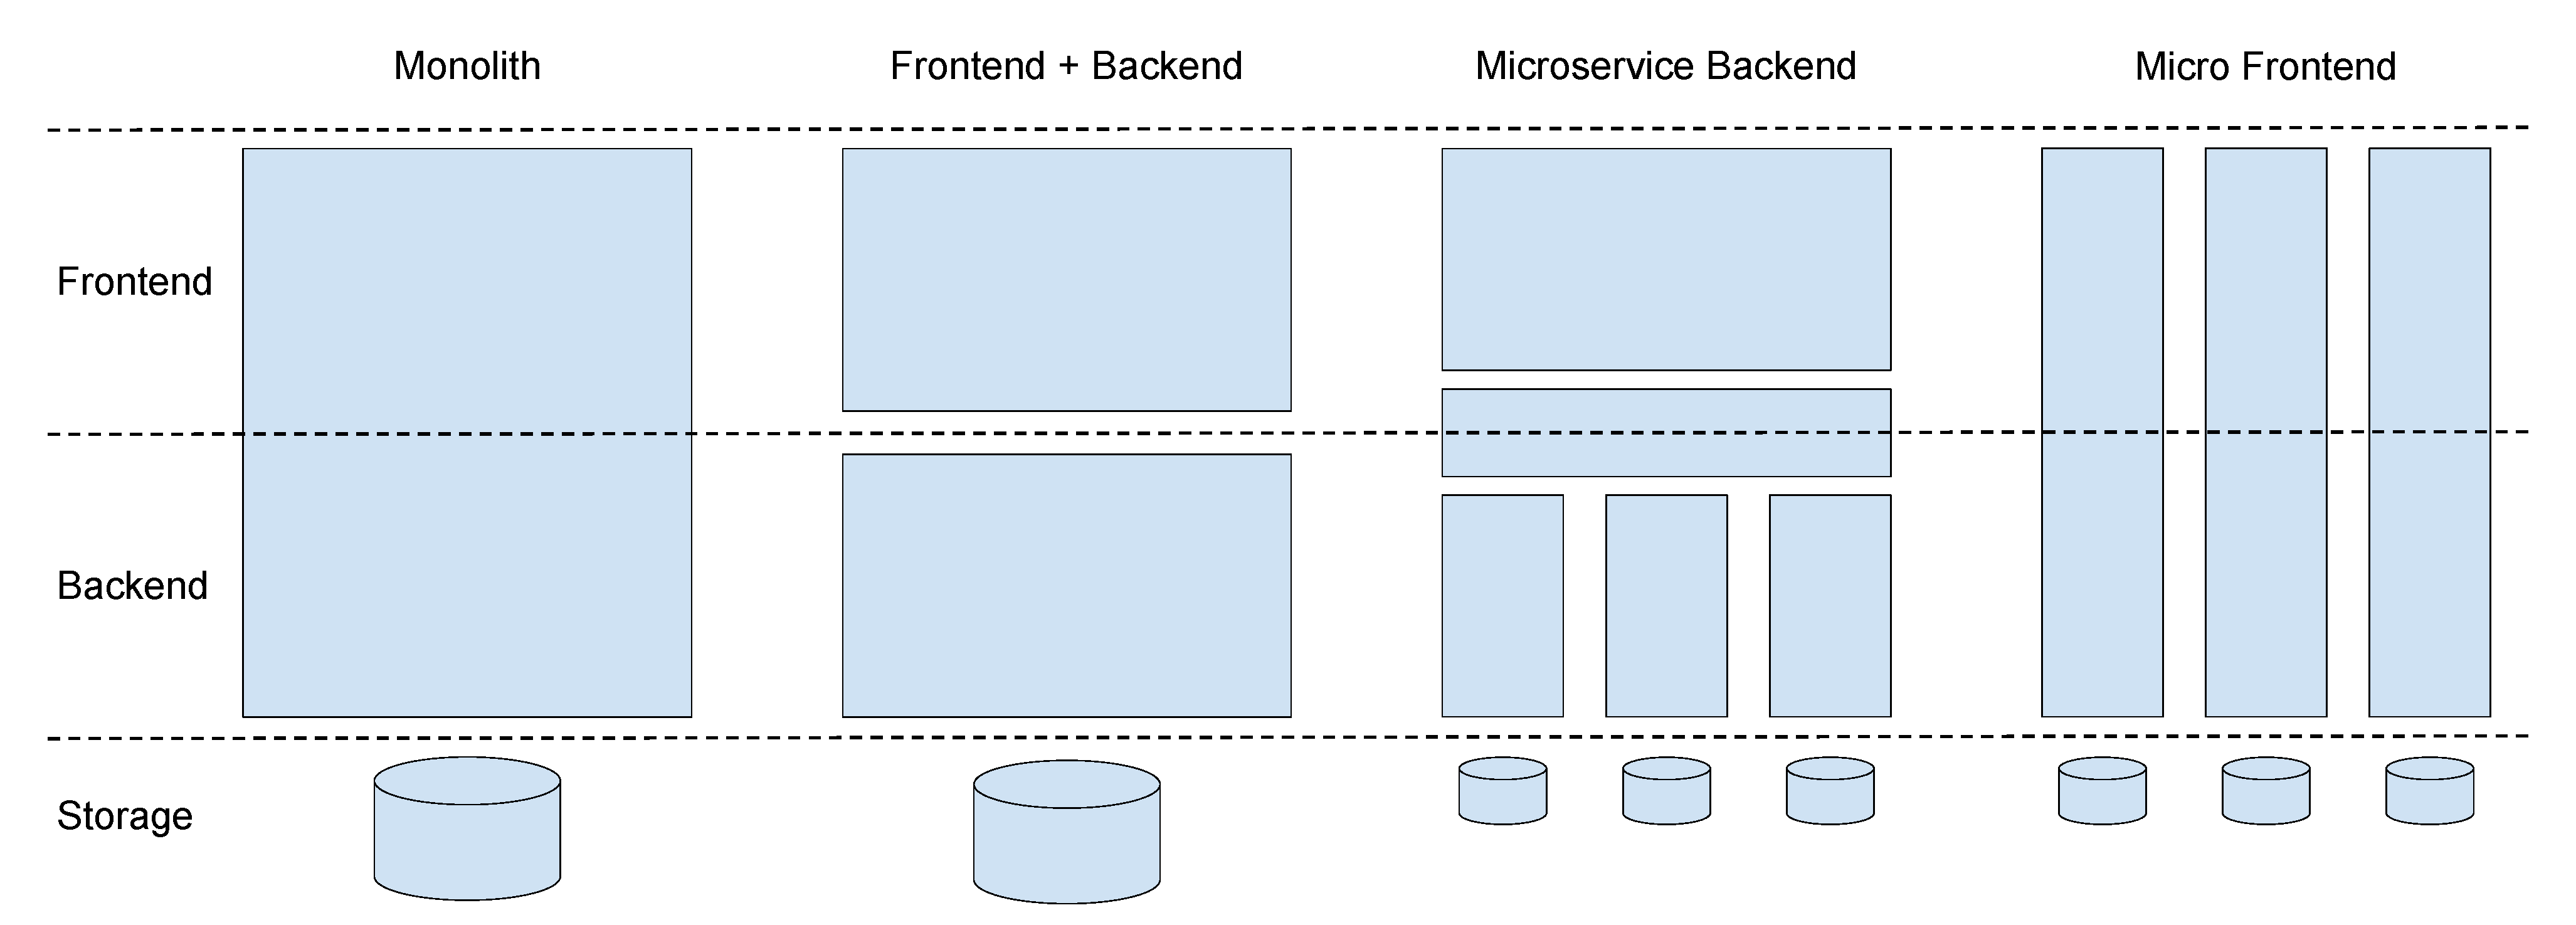
\includegraphics[width=\linewidth]{images/evolution-of-decomposition-strategies.pdf}
    \caption{An Evolution of Decomposition Strategies}
    \label{fig:evolution-of-decomposition-strategies}
\end{figure}

Even though \citeauthor{Geers2020} preferably envisions micro front-ends as fully vertically aligned with the back-end, that does not have to be the case. Many micro front-ends exist apply the architecture patterns of microservices, without being fully aligned with the back-end. Figure \ref{fig:micro-frontend-alignment} presents three approaches to aligning a micro front-end to a back-end. A \textit{Shallow Micro Front-end} is a micro front-end that is in no way aligned to the back-end. The back-end can be one monolith, microservices behind one API-Gateway or multiple services. Based on Conway's law, this probably also means that there exists development teams that work only on the back-end or only on the front-end \cites{Conway}. A \textit{Vertically Aligned Micro Front-end} is when there is a dedicated back-end service that the micro front-end primarily communicates with. A \textit{Monolithic Micro Front-end} is when a micro front-end is a part of a server side rendered monolith, where the back-end and front-end is delivered in one monolithic application. These ...

\begin{figure}
    \centering
    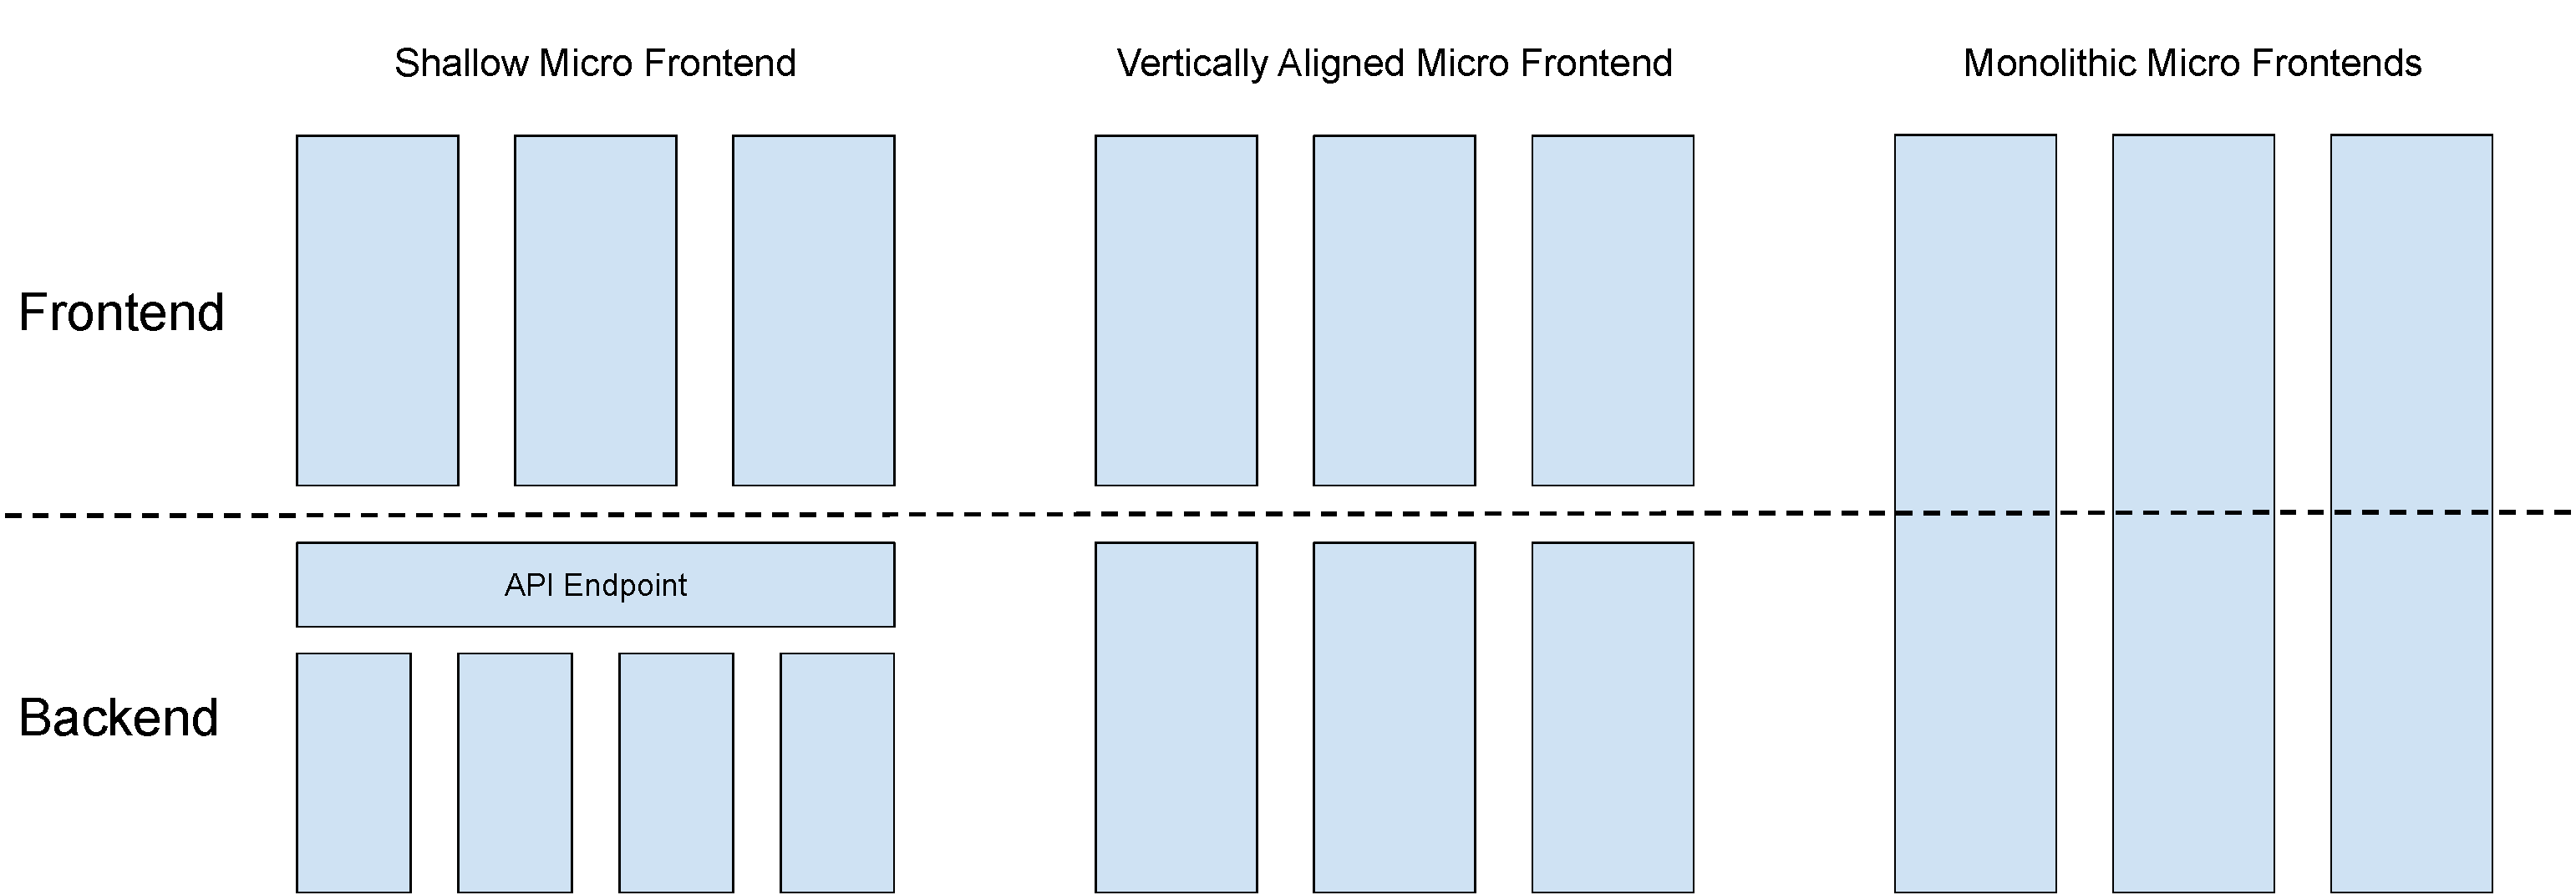
\includegraphics[width=\linewidth]{images/micro-frontend-strategies.pdf}
    \caption{Micro Front-end strategies}
    \label{fig:micro-frontend-alignment}
\end{figure}


\section{Pages and Fragments}

There are many different methods for composing micro front-ends into one coherent front-end. A very important distinction is also to differentiate between micro front-ends that are \textit{pages} or \textit{fragments}. All front-ends are composed by one or more pages. In this case a page refers to a full application view, that covers the full application window. A user can not view multiple pages simultaneously. A fragment is an element of a page. A fragment can be a button, a navigation bar or any other graphical components. A page can include many fragments.

Figure \ref{fig:fragment-page} exemplifies the concept. In this example, the front-end is composed of two pages, which can be served on two different routes. The pages are composed of fragments, and some of the fragments are identical on both pages.

\begin{figure}
    \centering
    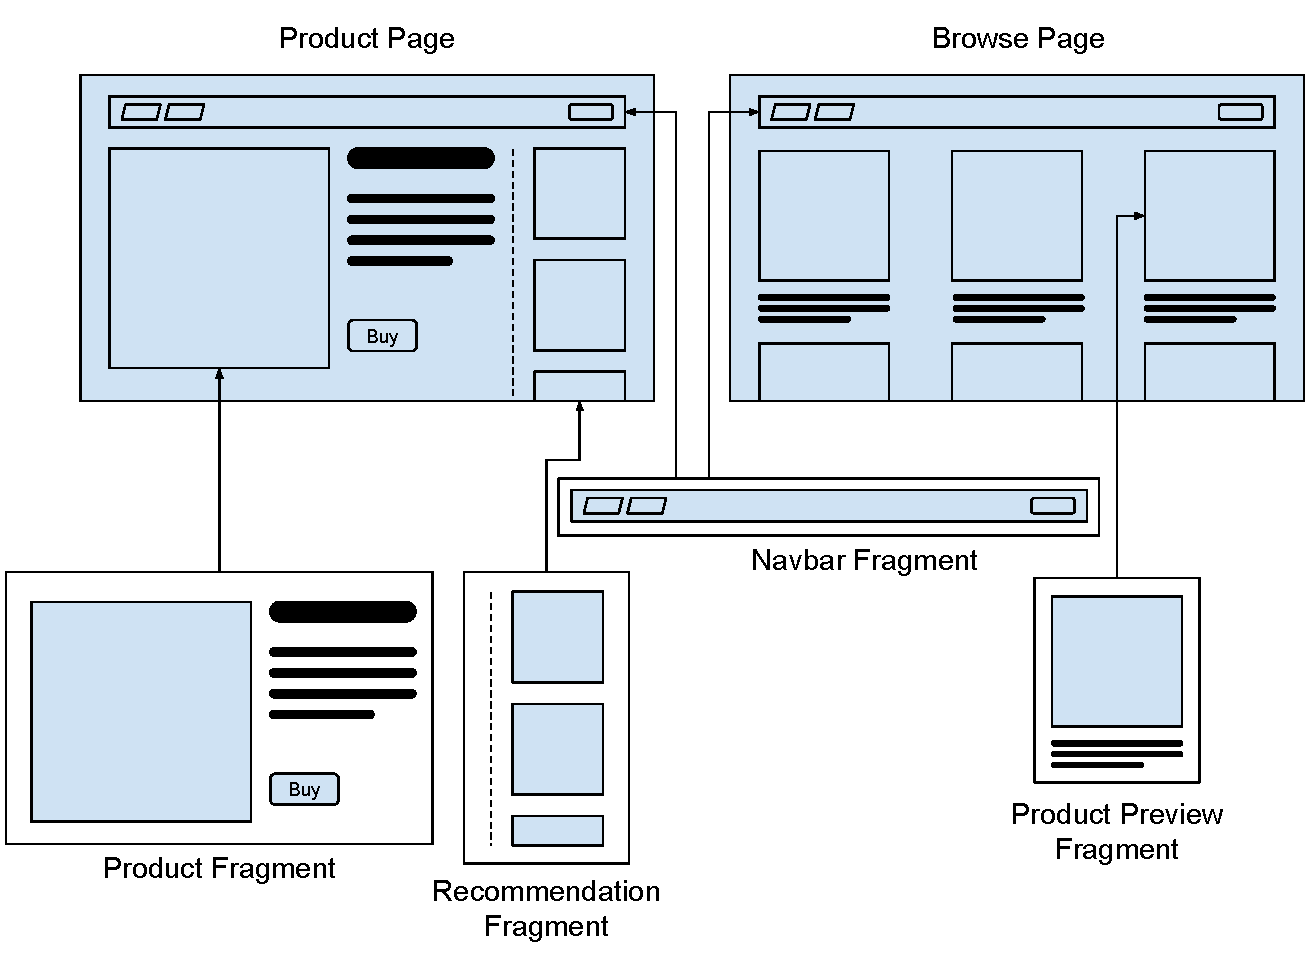
\includegraphics[width=0.9\linewidth]{images/fragment-page.pdf}
    \caption{An example of an e-commerce web page. It consists of two pages, and four fragments, where one fragment is reused on both pages.}
    \label{fig:fragment-page}
\end{figure}

The definition of a fragment is purposefully left vague as ``a part of a page''. The granularity is not specified, which means that multiple fragments in the example could be defined as one fragment, or that a fragment can be divided into multiple fragments. This also implies that a page is an edge case of one large complex fragment.

\section{Composing Micro Front-ends}

As a user uses an application the front-end has to be a coherent application, which means that different micro front-ends has to be integrated into a cohesive experience. Some differentiating questions that arise are ``when and where are the micro front-ends composed?'' The following sections aim to answer those questions. Note that micro front-end \textit{composition} is different from \textit{rendering}, which is when code is evaluated into HTML and CSS code. Composition is the process of integration multiple micro front-ends into one cohesive front-end.

\textbf{mention portlets}

\subsection{When are micro front-ends composed?}

Using ThoughtWorks definition of micro front-ends a micro front-end can be composed both in build-time and run-time \cites{Jackson2019}. Other definitions define micro front-ends as being composed in run-time \cite{Geers2020}. There exists a consensus that using build-time integration loses many of the benefits of using micro front-ends, like independent deployability \cite{Jackson2019}. It is also such a broad definition that most web pages could be defined as micro front-ends. For those reasons, only run-time composition will be considered.

\subsection{Where are micro front-ends composed?}

Micro front-ends can be integrated on the server, on the client, or a combination of both \cite{Jackson2019}. The simplest server side integration is to serve different web pages on different routes \cite{Jackson2019}. All traditional tools and processes can be used to develop the separate pages, and the different micro front-ends can be \acp{SPA}. This can be achieved with a web proxy to serve the different pages on a single domain address, which is visualized in Figure \ref{fig:web-proxy-example}.

\begin{figure}
    \centering
    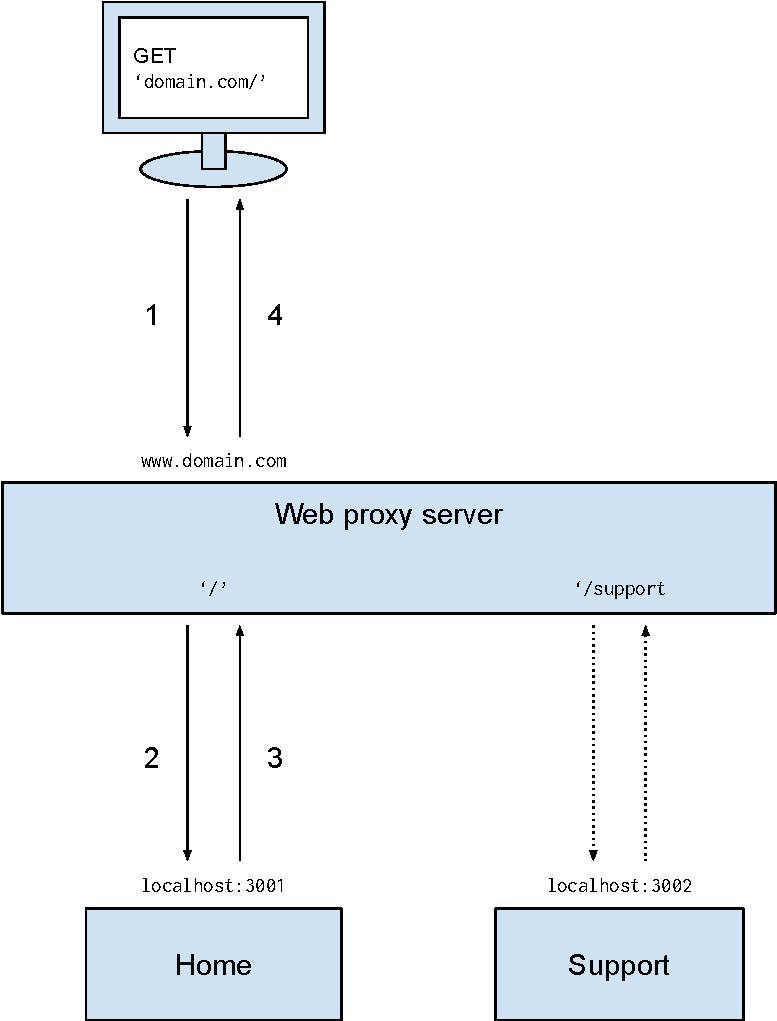
\includegraphics[width=0.5\linewidth]{images/web-proxy.pdf}
    \caption{A web proxy that redirects HTTP requests depending on the route requested. The web servers do can be developed with any existing mature web technology, without having to consider the other servers.}
    \label{fig:web-proxy-example}
\end{figure}

Server side integration can also be used to serve page fragments. This is sometimes called transclusion, and can be done by using technologies like Server Side Includes, Edge Side Includes, Zalando Tailor, or Podium \cite[ch.~4]{Geers2020}. Note that as pages just are large fragments, these technologies can also be used to divide an application on a page level.

All existing client side integration methods can be used for fragment composition, and therefore page composition. The most naive client side integration method is using iframes, which is a web-native standard \cite[ch.~2]{Geers2020}. Iframes were introduced with the HTML 4.01 standard in 1998 \cite{Raggett1999}, when web was still an early technology, which is why there are drawbacks to using them on a modern web app. The most notable trade-offs are performance overhead, accessibility problems, search engine optimization problems, and the lack of layout control \cite[ch.~2]{Geers2020}.

A much newer web-native standard is web components, which in practice is a suite of four web technology standards \cite{MDNWebDocs}. They allow dynamic custom elements to be defined and registered, in an encapsulated scope \cite{MDNWebDocs}. They are used by Google on large products like Youtube to include highly interactive elements \cite{ThePolymerProjectc}.

Figure \ref{fig:web-components} shows an example of how an example web component is created, defined, and what the \ac{DOM} is evaluated into. There are fewer drawbacks with using web components compared with using iframes, but some still exist. The largest issue is that web components do not server side rendering, as they have to be run in a browser at the client \cite[ch.~5]{Geers2020}. This issue can become a problem for performance, accessibility, and search engine optimization. Another drawback, compared with using build-time integration, is the lack of static annotations and analysis. Web components can be internally statically analyzed, but there does not exist any mechanism to share static annotations across the boundary of a web component.

\textbf{TODO: try to find academia about web components or custom elements}

\begin{figure}
\centering
\begin{subfigure}{.65\linewidth}
  \centering
\begin{lstlisting}[
basicstyle=\fontsize{7}{9}\selectfont\ttfamily,
breaklines=true,
frame=single
]
<html>
  <body>
    <my-component></my-component>

    <script>
class MyComponent extends HTMLElement {
  connectedCallback() {
    this.innerHTML = `<h1>Hello!</h1>`;
  }
}

customElements.define(
  'my-component',
  MyComponent
);
    </script>
  </body>
<html>
\end{lstlisting}
  \caption{An example of how to use custom elements. First the class \texttt{MyComponent} is defined, and registered on the name \texttt{my-component}. Then all instances of \texttt{my-component} is replaced on the \ac{DOM} with the custom element \texttt{MyComponent}.}
  \label{fig:sub1}
\end{subfigure}
\hfill
\begin{subfigure}{.30\linewidth}
  \centering
\begin{lstlisting}[
basicstyle=\fontsize{7}{9}\selectfont\ttfamily,
breaklines=true,
frame=single
]
<html>
  <body>
    <my-component>
      <h1>Hello!</h1>
    </my-component>
  </body>
<html>
\end{lstlisting}
  \caption{The result of how the custom element will be evaluated on the \ac{DOM}}
  \label{fig:sub2}
\end{subfigure}
\caption{An example of how to use custom elements which is a part of the Web Component technology suite. The left figure is evaluated to the right figure in run-time.}
\label{fig:web-components}
\end{figure}

As web components are a low-level construct, many frameworks exist that uses web components as a compilation target like Polymer, Stencil, SkateJS, Slim.js, hybrids, and snuggsi \cite{WebComponents.orgb}. Two of the most popular front-end frameworks, Angular \cite{Googlec} and Vue \cite{Vuejs}, has native support for being encapsulated as a web component. The potentially most popular front-end framework React does not natively output web components \cite{Dodson}. However, they do include documentation of how to wrap react components in a web component \cite{FacebookInc.}.

There exists micro front-end meta-frameworks that utilize other technologies than web components. Some of them are simple implementations like react-async-component that creates lazy loaded react components \cite{Matheson}. One of the most popular and extensive frameworks is single-spa \cite{Single-spa}. It is a shell application that includes other applications developed using other frameworks \cite{Single-spa}. Like a thin orchestration layer that handles routing and micro front end composition. This kind of framework has been called a unified single-page application, as it wraps other single-page-applications into one cohesive application \cite{Geers2020}. Single-spa requires that the root application be written as a single-spa application, which implies a considerable migration cost to existing applications \cite{Single-spa}. No micro front-end frameworks provide static analysis between the application boundaries.

\textbf{Summarize all technologies with a figure}

\section{Boundary Pushing Work}

\textbf{I know this is a bad title. What should I call this? It is for work that is being done which is amazing and boundary pushing (will redefine how micro front-ends are used), but not 100\% production ready or public yet.}

Mention Deja vu, Zalandos new framework, Module federation, and portals.

\textbf{WOW! https://github.com/runem/web-component-analyzer}